\begin{figure}[t]
\centering
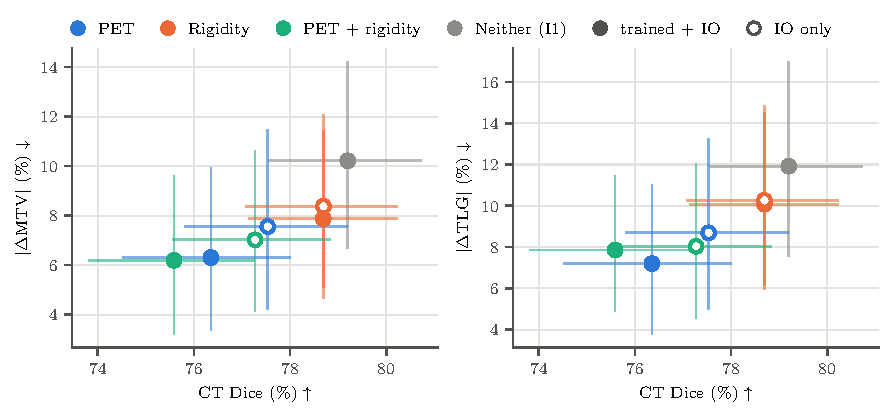
\includegraphics[width=\textwidth]{figures/q2.pdf}
\caption{Losses in training and IO versus only in IO (test set; CT Dice: 28 patients, PET: 26 patients). For each loss set, filled: network trained with the losses, then IO with them; hollow: network trained without them (T1), same IO. Grey: neither loss (I1). Points: patient means with 95\,\% patient-bootstrap confidence intervals for each method; confidence intervals for paired differences are reported in the text.}
\label{fig:q2}
\end{figure}
